\documentclass{jsarticle}
\usepackage[dvipdfmx]{graphicx}

\begin{document}
\section{目的}
    今回は, ~総務省, ~内閣府から公開されている統計データから,
    ~各都道府県間の情報格差について調べた.

    対象として, ~私たちが住む新潟の他に, ~大阪, ~山口, ~福岡,
    ~福島, ~長野, ~秋田, ~岐阜を選んだ.
    ~これらの都道府県は, ~班のメンバーのゆかりの地の他,
    ~新潟に面積が近い都道府県を選んだ.

\section{方法}
    調査方法として, ~主に授業内で配布されてデータを使用した.
    ~各県のブロードバンド接続率が情報格差に繋がっていると考え,
    ~様々なパラメータと比較をし, ~視覚化をした.
    ~主にメンバー全員でデータを調査し, ~まとめた.

    また, ~今回は全て平成26年度のデータを使用した.

\section{結果}
    以下に調査結果を示す.

    \subsection{所得と接続率}
        \begin{figure}[h]
            \begin{center}
                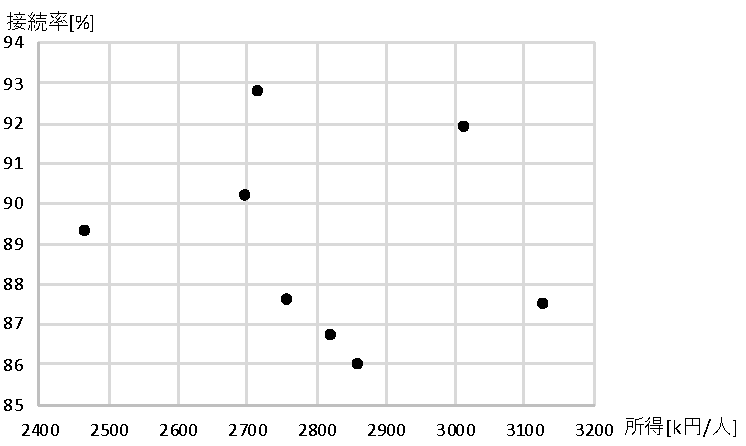
\includegraphics[width=10cm]{syotoku.pdf}
                \caption{所得-接続率散布図}
                \label{fig:所得}
            \end{center}     
        \end{figure}

        図\ref{fig:所得}は, ~各都道府県の所得と接続率を比較したものである.
        ~特に, ~法則性はみられない.

    \subsection{所得増加率と接続率}
        \begin{figure}[ht]
            \begin{center}
                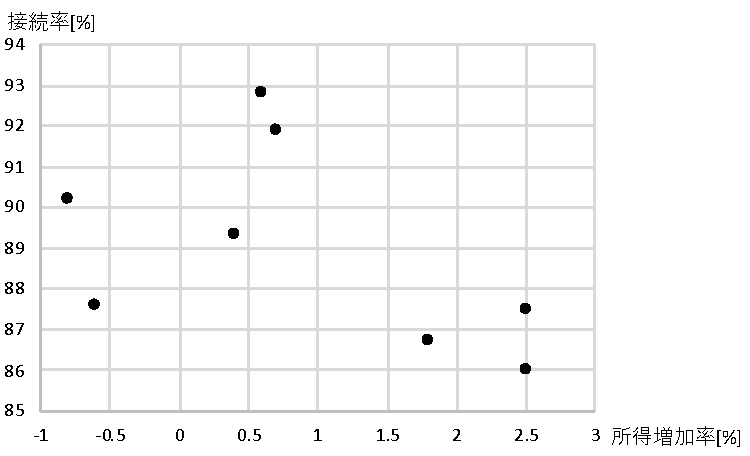
\includegraphics[width=10cm]{syotokuzouka.pdf}
                \caption{所得増加率-接続率散布図}
                \label{fig:所得増加率}
            \end{center}
        \end{figure}

        図\ref{fig:所得増加率}は, ~各都道府県の所得増加率と接続率を比較したものである.
        ~今回選択した都道府県を比べると,
        ~所得増加率が高いと接続率が低くなる傾向にみられる.

    \subsection{人口と接続率}
        \begin{figure}[ht]
            \begin{center}
                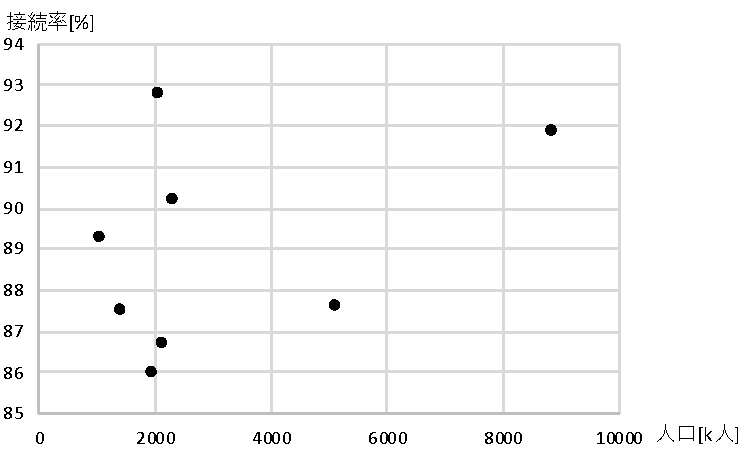
\includegraphics[width=10cm]{jinkou.pdf}
                \caption{人口-接続率散布図}
                \label{fig:人口}
            \end{center}
        \end{figure}

        図\ref{fig:人口}は, ~各都道府県の人口と接続率を比較したものである.
        ~今回選択した都道府県には, ~ほとんど人口の差がなく,
        ~あまり特徴は見つけられなかった.

    \subsection{人口増加率と接続率}
        \begin{figure}[ht]
            \begin{center}
                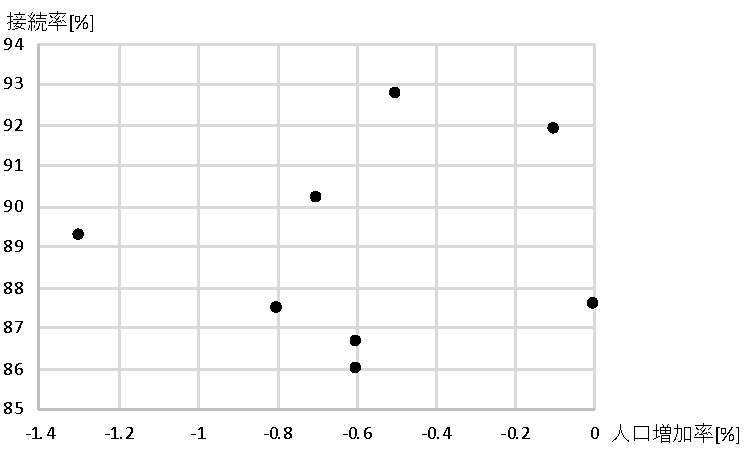
\includegraphics[width=10cm]{jinkouzouka.pdf}
                \caption{人口増加率-接続率散布図}
                \label{fig:人口増加}
            \end{center}
        \end{figure}

        図\ref{fig:人口増加}は, ~各都道府県の人口と接続率を比較したものである.
        ~図\ref{fig:人口}と同様に, ~特徴はみられなかった.

    \subsection{人口密度と接続率}
        配布資料に書かれてない情報として,
        ~各県の人口密度を調査してみた.

        これは, ~人口密度が高い都道府県,
        ~所謂都会に近い場所の方が接続率が高いと考えたからである.

        \begin{figure}[ht]
            \begin{center}
                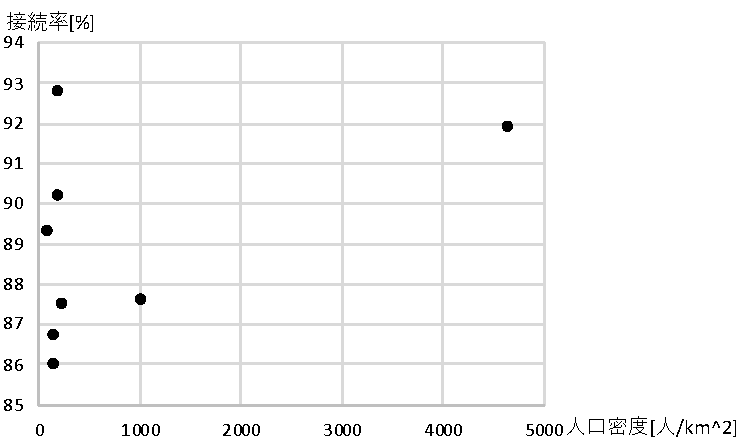
\includegraphics[width=10cm]{mitudo.pdf}
                \caption{人口密度-接続率散布図}
                \label{fig:人口密度}
            \end{center}
        \end{figure}

        図\ref{fig:人口密度}は, ~各都道府県の人口と接続率を比較したものである.
        上に書いた考察とはうって変わり,
        ~図\ref{fig:人口}よりも極端な偏りが見られる.

\section{考察 $\cdot$ 感想}
    各調査を通して, ~各項目と接続率とにはあまり関係性がみられないことがわかった.
    ~一つの原因として, ~比較する都道府県が少なかったことが考えられる.

    しかし, ~そもそも日本国内で明確に特徴が掴めるほど情報格差があるのかという疑問が残る.

    今回は統計データを元に調査を行なったが,
    ~インターネットなどでより情報格差について詳しく調べると,
    ~また違った発見があるのかもしれない.

\begin{thebibliography}{}
    \bibitem{handout} 2019-Ec3計算機システム資料(5)
\end{thebibliography}
\end{document}